%%%%%%%%%%%%%%%%%%%%%%%%%%%%%%%%%%%%%%%%%%%%%%%%%%%%%%%%%%%%%%%%
%%                                                            %%
%% aGreekPrimer, Italian translation 2016.12 - 2017           %%
%%                                                            %%
%% From:  Clarence W. Gleason, A Greek Primer                 %%
%%        (1903, New York, American Book Company)             %%
%%                                                            %%
%%        https://archive.org/details/greekprimer00glea       %%
%%                                                            %%
%% Translated by g.p.ciceri <gp.ciceri@gmail.com>             %%
%% ---------------------------------------------------------- %%
%% This translation is Licensed under                         %%
%% Creative Commons Attribution-ShareAlike 4.0 International  %%
%% https://creativecommons.org/licenses/by-sa/4.0/            %%
%%                                                            %%
%%%%%%%%%%%%%%%%%%%%%%%%%%%%%%%%%%%%%%%%%%%%%%%%%%%%%%%%%%%%%%%%

% ᾶῖῶῆῦ  
% ἀἰὐἐὀὠἠ 
% ὰὲὶὸὺὼὴ 
% ἁἱὑὁὡἡῥ
% άέίόύήώΆΉ
% ἂἒὒἲὂὢἢὒἚἊ
% ἃἳὓὃἣὣἓἋἛ
% ἄἔἴὄὔὤἤἌἬ
% ἅἕἵὅὕὥἥἍἭ
% ἆὦἶἦὖἯἏὯἇὧἷἧὗἯἏὯ 

% ᾳῃῳ
% ᾱῑῡ
% ᾀᾐᾠ
% ᾰῐῠ
% ᾂᾒᾢ
% ϊ ϋ
% ᾄᾔᾤ
% ΰ ΐ
% ᾆᾖᾦ
% ᾲῂῲ
% ᾴῄῴ
% ᾷῇῷ
% ᾳῃῳ
% ᾱῑῡ
% ᾰῐῠ

% āēīōū
% ăĕĭŏŭ

% ᾳῃῳ
% ᾷῇῷ


\documentclass[nols]{tufte-handout}

%\geometry{showframe} % display margins for debugging page layout

\usepackage{fontspec}
\usepackage{ifxetex}
\setmainfont[Path=./fonts/palatino-linotype/, ItalicFont=palai.ttf, BoldFont=palab.ttf]{pala.ttf}
%\setmainfont[Path=./fonts/GFS_Didot/, ItalicFont=GFSDidotItalic.ttf, BoldFont=GFSDidotBold.ttf]{GFSDidot.ttf}

\newfontfamily\GFSDidotBf[Path=./fonts/GFS_Didot/]{GFSDidotBold.ttf}
\newfontfamily\GFSDidot[Path=./fonts/GFS_Didot/]{GFSDidot.ttf}

\newcommand{\didobf}[1]{{\GFSDidotBf #1}}
\newcommand{\dido}[1]{{\GFSDidot #1}}


\usepackage{lipsum}
\usepackage{url}
\usepackage{longtable}
\usepackage{stackengine}

\usepackage{graphicx} % allow embedded images
  \setkeys{Gin}{width=\linewidth,totalheight=\textheight,keepaspectratio}
  \graphicspath{{graphics/}} % set of paths to search for images
\usepackage{amsmath}  % extended mathematics
\usepackage{booktabs} % book-quality tables
\usepackage{units}    % non-stacked fractions and better unit spacing
\usepackage{multicol} % multiple column layout facilities
\usepackage{lipsum}   % filler text
\usepackage{fancyvrb} % extended verbatim environments
  \fvset{fontsize=\normalsize}% default font size for fancy-verbatim environments

% Standardize command font styles and environments
\newcommand{\doccmd}[1]{\texttt{\textbackslash#1}}% command name -- adds backslash automatically
\newcommand{\docopt}[1]{\ensuremath{\langle}\textrm{\textit{#1}}\ensuremath{\rangle}}% optional command argument
\newcommand{\docarg}[1]{\textrm{\textit{#1}}}% (required) command argument
\newcommand{\docenv}[1]{\textsf{#1}}% environment name
\newcommand{\docpkg}[1]{\texttt{#1}}% package name
\newcommand{\doccls}[1]{\texttt{#1}}% document class name
\newcommand{\docclsopt}[1]{\texttt{#1}}% document class option name
\newenvironment{docspec}{\begin{quote}\noindent}{\end{quote}}% command specification environment

% concetti morfosintattici
\usepackage{xspace} 
\newcommand{\noun}{\textsc{sostantivo}\xspace}
\newcommand{\nouns}{\textsc{sostantivi}\xspace}
\newcommand{\adject}{\textsc{aggettivo}\xspace}
\newcommand{\adjects}{\textsc{aggettivi}\xspace}
\newcommand{\gnumber}{\textsc{numero}\xspace}
\newcommand{\gnumbers}{\textsc{numeri}\xspace}
\newcommand{\gender}{\textsc{genere}\xspace}
\newcommand{\genders}{\textsc{generi}\xspace}
\newcommand{\gcase}{\textsc{caso}\xspace}
\newcommand{\gcases}{\textsc{casi}\xspace}
\newcommand{\tense}{\textsc{tempo}\xspace}
\newcommand{\mood}{\textsc{modo}\xspace}
\newcommand{\gverb}{\textsc{verbo}\xspace}
\newcommand{\gverbs}{\textsc{verbi}\xspace}
\newcommand{\adjective}{\textsc{aggettivo}\xspace}
\newcommand{\nom}{\textsc{nom}\xspace}
\newcommand{\gen}{\textsc{gen}\xspace}
\newcommand{\dat}{\textsc{dat}\xspace}
\newcommand{\acc}{\textsc{acc}\xspace}
\newcommand{\voc}{\textsc{voc}\xspace}
\newcommand{\gexit}{\textsc{uscita}\xspace}
\newcommand{\gexits}{\textsc{uscite}\xspace}
\newcommand{\declinazione}{\textsc{declinazione}\xspace}
\newcommand{\masc}{\textsc{maschile}\xspace}
\newcommand{\femm}{\textsc{femminile}\xspace}
\newcommand{\neut}{\textsc{neutro}\xspace}

\newcommand{\indic}{\textsc{indicativo}\xspace}
\newcommand{\imper}{\textsc{imperativo}\xspace}
\newcommand{\gcong}{\textsc{congiuntivo}\xspace}
\newcommand{\ott}{\textsc{ottativo}\xspace}
\newcommand{\partic}{\textsc{participio}\xspace}
\newcommand{\infin}{\textsc{infinito}\xspace}

\newcommand{\pres}{\textsc{presente}\xspace}
\newcommand{\imperf}{\textsc{imperfetto}\xspace}
\newcommand{\aor}{\textsc{aoristo}\xspace}
\newcommand{\fut}{\textsc{futuro}\xspace}
\newcommand{\perf}{\textsc{perfetto}\xspace}
\newcommand{\pperf}{\textsc{piuccheperfetto}\xspace}

\newcommand{\sing}{\textsc{singolare}\xspace}
\newcommand{\plur}{\textsc{plurale}\xspace}
\newcommand{\dual}{\textsc{duale}\xspace}

\newcommand{\si}{\textsc{sing}\xspace}
\newcommand{\pl}{\textsc{plur}\xspace}
\newcommand{\du}{\textsc{dual}\xspace}

\newcommand{\att}{\textsc{attivo}\xspace}
\newcommand{\med}{\textsc{medio}\xspace}
\newcommand{\pass}{\textsc{passivo}\xspace}
\newcommand{\medpass}{\textsc{medio-passivo}\xspace}


% italianitudini
\renewcommand{\figurename}{Figura}
\renewcommand{\tablename}{Tabella}
\renewcommand{\contentsname}{Indice}

% fix per un qualche problema
\ifxetex
  \newcommand{\textls}[2][5]{%
    \begingroup\addfontfeatures{LetterSpace=#1}#2\endgroup
  }
  \renewcommand{\allcapsspacing}[1]{\textls[15]{#1}}
  \renewcommand{\smallcapsspacing}[1]{\textls[10]{#1}}
  \renewcommand{\allcaps}[1]{\textls[15]{\MakeTextUppercase{#1}}}
  \renewcommand{\smallcaps}[1]{\smallcapsspacing{\scshape\MakeTextLowercase{#1}}}
  \renewcommand{\textsc}[1]{\smallcapsspacing{\textsmallcaps{#1}}}
\fi

% too many float...
\extrafloats{100}

\title{A Greek Primer. Introduzione al Greco Antico \newline Lezione XIV - Temi in Palatale e in Labiale della Declinazione in Consonante.}

\author[gpciceri]{a cura di Milagathòs: Milo's help to enjoy humanities}

\date{16 Gennajo 2017} % without \date command, current date is supplied


\begin{document}

\maketitle% this prints the handout title, author, and date

\begin{marginfigure}[-2.0cm]
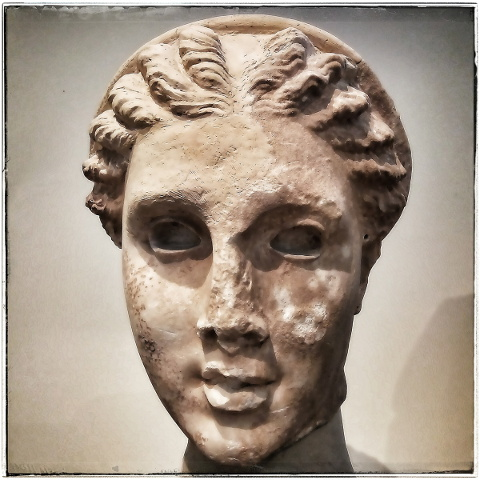
\includegraphics{smallthumb-lesson_XIII.jpeg}
\setfloatalignment{b}
\end{marginfigure}


\begin{abstract}
\noindent
Queste lezioni si articolano in \textsc{elementi grammaticali}, 
espressi sommariamente, seguiti da \textsc{vocabolari} per il lessico di base 
e da \textsc{frasi da tradurre} dal greco e in greco. 
\
L'approccio è quello del testo-laboratorio di morfosintassi: 
si presenta punto per punto - riprendendone la numerazione - 
l'esposizione di Gleason\cite{gleason1903}.\\
\bigskip
\noindent
Lezione XIV: temi in Palatale e in Labiale della Declinazione in Consonante (Terza Declinazione); vocabolario, esercizi.
\end{abstract}

%\printclassoptions

\newthought{161.} La \textbf{Terza Declinazione} o \textbf{Declinazione in consonante} comprende tutti i nomi che non appartengono alle altre due.
Il tema di questi nomi di solito \textit{termina in consonante}, ma ci sono anche, pochi, temi che \textit{terminano in vocale o dittongo}. 

\newthought{162. Modelli}

\begin{fullwidth}
\begin{table}[!htbp]
  \centering
  \begin{tabular}{l l l l l l l}
    %\toprule
	\multicolumn{7}{c}{\textsc{III Declinazione - Temi in Palatale e in Labiale}} \\
	& \didobf{φύλαξ, ὁ,} & \didobf{διῶρυξ, ἡ,} & \didobf{κλώψ, ὁ,} & \hspace{10 mm} & \multicolumn{2}{c}{\textsc{Termin. Masc. e Femm.}} \\
	& \multicolumn{1}{c}{\textit{guardia}}
	& \multicolumn{1}{c}{\textit{canale}}
	& \multicolumn{1}{c}{\textit{ladro}}
	& \hspace{10 mm}
	& \multicolumn{1}{l}{\textsc{Greco}} & \multicolumn{1}{l}{\textsc{Latino}} \\
   
	\multicolumn{7}{c}{\textsc{singolare}} \\
    \textsc{n.} & \didobf{φύλαξ}   & \didobf{διῶρυξ}   & \didobf{κλώψ}   & \hspace{10 mm} & \didobf{ς} o \textemdash & s o \textemdash \\
    \textsc{g.} & \didobf{φύλακος} & \didobf{διώρυχος} & \didobf{κλωπός} & \hspace{10 mm} & \didobf{ος}              & is \\
    \textsc{d.} & \didobf{φύλακι}  & \didobf{διώρυχι}  & \didobf{κλωπί}  & \hspace{10 mm} & \didobf{ι}               & ī \\
	\textsc{a.} & \didobf{φύλακα}  & \didobf{διώρυχα}  & \didobf{κλώπα}  & \hspace{10 mm} & \didobf{α} o \didobf{ν}  & em, im \\
	\textsc{v.} & \didobf{φύλαξ}   & \didobf{διῶρυξ}   & \didobf{κλώψ}   & \hspace{10 mm} & \didobf{ς} o \textemdash & s o \textemdash \\
	
	\multicolumn{7}{c}{\textsc{plurale}} \\
	\textsc{n.v.} & \didobf{φύλακες} & \didobf{διώρυχες} & \didobf{κλῶπες} & \hspace{10 mm} & \didobf{ες}            & ēs     \\
    \textsc{g.}   & \didobf{φυλάκων} & \didobf{διωρύχων} & \didobf{κλωπῶν} & \hspace{10 mm} & \didobf{ων}            & um     \\
    \textsc{d.}   & \didobf{φύλακι}  & \didobf{διώρυξι}  & \didobf{κλωψί}  & \hspace{10 mm} & \didobf{σι}            & ibus   \\
	\textsc{a.}   & \didobf{φύλακας} & \didobf{διώρυχας} & \didobf{κλῶπας} & \hspace{10 mm} & \didobf{ας (νς)}       & ēs, īs \\
    %\bottomrule
  \end{tabular}
  \label{tab:normaltab}
  %\zsavepos{pos:normaltab}
\end{table}
\end{fullwidth}

\newthought{Osservazioni}
\begin{itemize}
\item[\textsc{1.}] Nota le similitudini tra le terminazioni greche e le corrispondenti latine. 
\item[\textsc{2.}] Osserva come nel \nom \sing e nel \dat \plur la \didobf{ς} si combina con la muta finale del tema per formare una \didobf{ξ} o una \didobf{ψ}. 
Una muta labiale (\didobf{π, β, φ}) con la \didobf{ς} forma una \didobf{ψ}, una muta palatale (\didobf{κ, γ, χ}) forma una \didobf{ξ}.
\item[\textsc{3.}] Anche in questa declinazione l'accento rimane per quanto possibile sulla sillaba su cui si trova al \nom \sing; 
ma nei monosillabi, come in \didobf{κλώψ}, si accenta l'ultima nel \gen e nel \dat di tutti i numeri; \didobf{-ων} e \didobf{-οιν} hanno accento circonflesso.
\end{itemize}


\newthought{163. Vocabolario}

\begin{multicols}{2}
    \noindent \hangindent=1em \didobf{διῶπυξ, διώρυχος, ἡ} \textit{canale}.  \\
    \noindent \hangindent=1em \didobf{ἕργον, τό} \textit{lavoro, compito}.  \\
    \noindent \hangindent=1em \didobf{Θρᾷξ, Θρᾳκός, ὁ} \textit{un trace (abitante della Tracia)}.  \\
    \noindent \hangindent=1em \didobf{κῆρυξ, κήρυκος, ὁ} \textit{araldo}.     \\
    \noindent \hangindent=1em \didobf{κλώψ, κλωπός, ὁ} \textit{ladro}.  \\
    \noindent \hangindent=1em \didobf{πέρδιξ, πέρδικος, ὁ, ἡ} \textit{pernice}.  \\
    \noindent \hangindent=1em \didobf{φάλαγξ, φάλαγγος, ἡ} \textit{linea di battaglia}.  \\
	
    \noindent \hangindent=1em \didobf{φύλαξ, φύλακος, ὁ} \textit{guardia}.  \\
	
	\noindent \hangindent=1em \didobf{ἕκαστος, η, ον} agg. \textit{ogni}.  \\
    \noindent \hangindent=1em \didobf{ἐμός, ή, όν} pron.poss. \textit{mio}.  \\
	
	\noindent \hangindent=1em \didobf{πιστός, ή, όν} agg. \textit{fedele, leale}.  \\
	\noindent \hangindent=1em \didobf{ῥᾴδιος, α, ον} agg.  \textit{facile}.  \\
	
	\noindent \hangindent=1em \didobf{πρό} prep. con \gen \textit{in fronte a}, \textit{prima di}.  \\
	
\end{multicols}


\newthought{164. Traduci:}
\textsc{1.}~\dido{μισθὸν ἡμερῶν δέκα ἑκάστῳ τῶν Θρᾳκῶν πέμψει.} \quad
\textsc{2.}~\dido{ἐστράτευκα γὰρ πολλοὺς παρασάγγας διὰ τῆς τῶν πολεμίων χώρας.} \quad
\textsc{3.}~\dido{ἐντεῦθεν δὲ οἱ κήρυκες ἤγαγον τὰς ἐπιστολὰς παρὰ τὸν στρατεγόν.} \quad
\textsc{4.}~\dido{τίς, ὦ κῆρυξ, ἄξει τὴν φάλαγγα;} \quad
\textsc{5.}~\dido{ἐκ δὲ τῆς σκηνῆς ἔφυγεν ὁ πελταστὴς παρὰ τὴν διώρυχα.} \quad
\textsc{6.}~\dido{παρὰ δὲ τῇ διώρυχι οἱ πιστοὶ φύλακες ἔμενον.} \quad
\textsc{7.}~\dido{οἱ δὲ νεανίαι ἐθήρευσαν πέρδικας ἐν τῷ πεδίῳ.} \quad
\textsc{8.}~\dido{ἐπεὶ δὲ πρὸ τῶν οἰκιῶν ἦσαν, κλῶπες ἥρπασαν τὰ ὅπλα.} \quad
\textsc{9.}~\dido{οὐ γὰρ ῥᾴδιον ἦν ἔργον διώκειν τοὺς πολεμίους.} \quad
\textsc{10.}~\dido{εἰ δικαίους νόμους ἔχουσι, καλῶς ἔχει.}

\newthought{165. Scrivi in Greco:}
\textsc{1.}~Le guardie persuasero i ladri a fuggire. \quad
\textsc{2.}~Se mio fratello ha mandato la lettera, è stato leale. \quad
\textsc{3.}~Parlò bene, ma noi non imparammo. \quad

\begin{figure}[!b]
  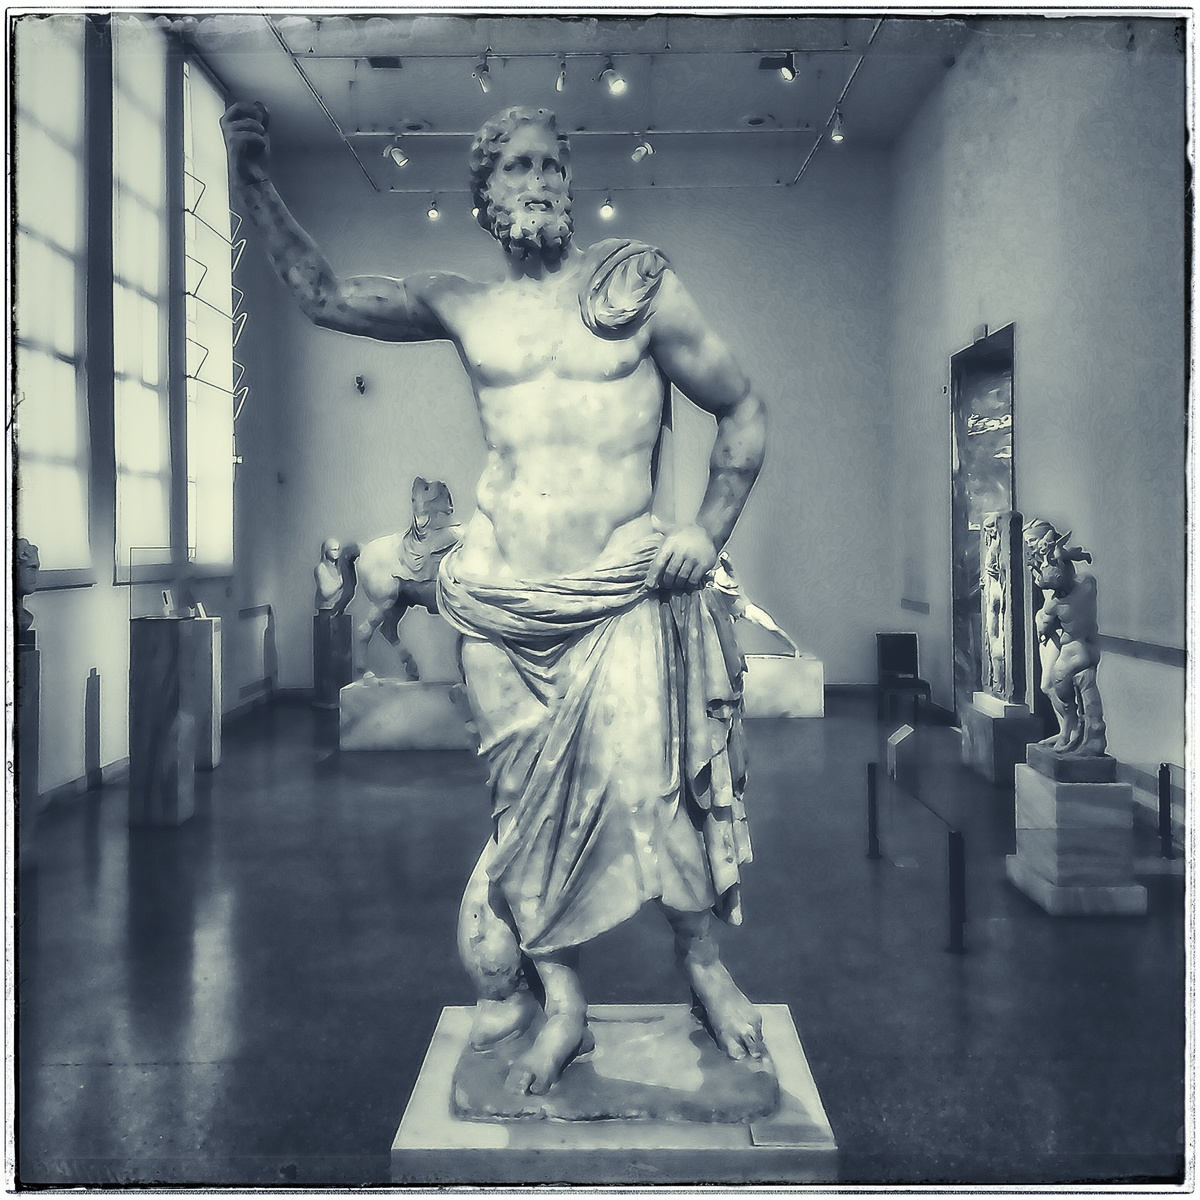
\includegraphics[width=0.45\linewidth]{thumb-lesson_XIV.jpeg}
  \caption{Museo Nazionale di Archeologia di Atene}
  \label{fig:textfig}
  %\zsavepos{pos:textfig}
  %\setfloatalignment{b}
\end{figure}

 

\nobibliography{greekBiblio}
\bibliographystyle{alpha}


\end{document}
